%!TEX program = xelatex
\documentclass[dvipsnames, svgnames,a4paper,11pt]{article}
% ----------------------------------------------------
%   中山大学物理与天文学院本科实验报告模板
%   作者:Huanyu Shi,2019级
%   知乎:https://www.zhihu.com/people/za-ran-zhu-fu-liu-xing
%   Github:https://github.com/Huanyu-Shi/SYSU-SPA-Labreport-Template
%   Last update : 2023.4.10
% ----------------------------------------------------

% ----------------------------------------------------- 
%	加边框的命令
%	参考:https://tex.stackexchange.com/questions/531559/how-to-add-the-page-border-for-first-two-pages-in-latex
\usepackage{tikz}
\usetikzlibrary{calc}
\usepackage{eso-pic}
\AddToShipoutPictureBG{%
\begin{tikzpicture}[overlay,remember picture]
\draw[line width=0.6pt] % 边框粗细
    ($ (current page.north west) + (0.6cm,-0.6cm) $)
    rectangle
    ($ (current page.south east) + (-0.6cm,0.6cm) $); % 边框位置
\end{tikzpicture}}


\usepackage{xcolor}
\definecolor{c1}{HTML}{2752C9} % 目录颜色
\definecolor{c2}{RGB}{190,20,83} % 引用颜色

\usepackage{ctex}
\usepackage[top=28mm,bottom=28mm,left=15mm,right=15mm]{geometry}
\usepackage{hyperref} 
\hypersetup{
	colorlinks,
	linktoc = section, % 超链接位置,选项有section, page, all
	linkcolor = c1, % linkcolor 目录颜色
	citecolor = c1  % citecolor 引用颜色
}
\usepackage{amsmath,enumerate,multirow,float}
\usepackage{tabularx}
\usepackage{tabu}
\usepackage{subfig}
\usepackage{fancyhdr}
\usepackage{graphicx}
\usepackage{wrapfig}  
\usepackage{physics}
\usepackage{appendix}
\usepackage{amsfonts}

%
\usepackage{tcolorbox}
\tcbuselibrary{skins,breakable}
\newtcolorbox{tbox}[2][]{
    colframe=black!70!,
    breakable,
    enhanced,
	boxrule =0.5pt,
    title = {#2},
    fonttitle = \large\kaishu\bfseries,
	drop fuzzy shadow,
    #1
}
\newtcolorbox[auto counter,number within=section]{question}[1][]{
  top=2pt,bottom=2pt,arc=1mm,
  boxrule=0.5pt,
%   frame hidden,
  breakable,
  enhanced, %跨页后不会显示下边框
  coltitle=c1!80!gray,
  colframe=c1,
  colback=c1!3!white,
  drop fuzzy shadow,
  title={思考题~\thetcbcounter:\quad},
  fonttitle=\bfseries,
  attach title to upper,
  #1
}
\newcommand{\setLhead}[1]{%
  \lhead{{\color{gray}\kaishu #1}} % 定义新的命令,设置右边页眉的内容
}
\newcommand{\setRhead}[1]{%
  \rhead{{\color{gray}\kaishu #1}} % 定义新的命令,设置右边页眉的内容
}
% ---------------------------------------------------------------------
%	利用cleveref改变引用格式,\cref是引用命令
\usepackage{cleveref}
\crefformat{figure}{#2{\textcolor{c2}{图 #1}}#3} % 图片的引用格式
\crefformat{equation}{#2{(\textcolor{c2}{#1})}#3} % 公式的引用格式
\crefformat{table}{#2{\textcolor{c2}{表 #1}}#3} % 表格的引用格式


% ---------------------------------------------------------------------
%	页眉页脚设置
\fancypagestyle{plain}{\pagestyle{fancy}}
\pagestyle{fancy}
\setLhead{中山大学物理与天文学院基础物理实验预习报告}
%\lhead{\kaishu 中山大学物理与天文学院物理实验\uppercase\expandafter{\romannumeral3}} % 左边页眉,学院 + 课程
%\rhead{{\color{gray}\kaishu Template 实验报告模板}} % 右边页眉,实验报告标题
\setRhead{实验1\hspace{1pt}冰的熔化热测量}
\cfoot{\thepage} % 页脚,中间添加页码


% ---------------------------------------------------------------------
%	对目录、章节标题的设置
\renewcommand{\contentsname}{\centerline{\huge 目录}}
\usepackage{titlesec}
\usepackage{titletoc}
% \titleformat{章节}[形状]{格式}{标题序号}{序号与标题间距}{标题前命令}[标题后命令]
\titleformat{\section}{\centering\LARGE\songti}{}{1em}{}

% ---------------------------------------------------------------------
%   listing代码环境设置
\usepackage{listings}
\lstloadlanguages{python}
\lstdefinestyle{pythonstyle}{
backgroundcolor=\color{gray!5},
language=python,
frameround=tftt,
frame=shadowbox, 
keepspaces=true,
breaklines,
columns=spaceflexible,                   
basicstyle=\ttfamily\small, % 基本文本设置,字体为teletype,大小为scriptsize
keywordstyle=[1]\color{c1}\bfseries, 
keywordstyle=[2]\color{Red!70!black},   
stringstyle=\color{Purple},       
showstringspaces=false,
commentstyle=\ttfamily\scriptsize\color{green!40!black},%注释文本设置,字体为sf,大小为smaller
tabsize=2,
morekeywords={as},
morekeywords=[2]{np, plt, sp},
numbers=left, % 代码行数
numberstyle=\it\tiny\color{gray}, % 代码行数的数字字体设置
stepnumber=1,
rulesepcolor=\color{gray!30!white}
}




% ---------------------------------------------------------------------
%	其他设置
\def\degree{${}^{\circ}$} % 角度
\graphicspath{{./images/}} % 插入图片的相对路径
\allowdisplaybreaks[4]  %允许公式跨页 % 导入模板的相关设置
\usepackage{lipsum}
\usepackage{indentfirst}
\usepackage{pdfpages}
\usepackage{multirow}
\usepackage{subfig}
\usepackage{graphicx}
\usepackage{float} 
\renewcommand{\d}{\mathrm{d}}


%---------------------------------------------------------------------
%	正文
%---------------------------------------------------------------------
\setRhead{实验BD1\ 复摆与混沌}%实验名称
\begin{document}


\begin{table}
	\renewcommand\arraystretch{1.7}
	\begin{tabularx}{\textwidth}{
		|X|X|X|X
		|X|X|X|X|}
	\hline
	\multicolumn{2}{|c|}{预习报告}&\multicolumn{2}{|c|}{实验记录}&\multicolumn{2}{|c|}{分析讨论}&\multicolumn{2}{|c|}{总成绩}\\
	\hline
	 & &  & &  & &  & \\
	\hline
	\end{tabularx}
\end{table}


\begin{table}
	\renewcommand\arraystretch{1.7}
	\begin{tabularx}{\textwidth}{|X|X|X|X|}
	\hline
	专业:& 物理学类 &年级:& 2023级\\
	\hline
	姓名:& 姚昊廷  & 学号:&22322091\\
	\hline
	实验时间:& 2024.9.26& 教师签名:& \\
	\hline
	\end{tabularx}
\end{table}

\begin{center}
	\LARGE 实验BD1\ 复摆与混沌
\end{center}

\textbf{【实验报告注意事项】}
\begin{enumerate}
	\item 实验报告由三部分组成:
	\begin{enumerate}
		\item 预习报告:(提前一周)认真研读\underline{\textbf{实验讲义}},弄清实验原理;实验所需的仪器设备、用具及其使用(强烈建议到实验室预习),完成课前预习思考题;了解实验需要测量的物理量,并根据要求提前准备实验记录表格(第一循环实验已由教师提供模板,可以打印)。预习成绩低于10分(共20分)者不能做实验。
	    \item 实验记录:认真、客观记录实验条件、实验过程中的现象以及数据。实验记录请用珠笔或者钢笔书写并签名(\textcolor{red}{\textbf{用铅笔记录的被认为无效}})。\textcolor{red}{\textbf{保持原始记录,包括写错删除部分,如因误记需要修改记录,必须按规范修改。}}(不得输入电脑打印,但可扫描手记后打印扫描件);离开前请实验教师检查记录并签名。
	    \item 分析讨论:处理实验原始数据(学习仪器使用类型的实验除外),对数据的可靠性和合理性进行分析;按规范呈现数据和结果(图、表),包括数据、图表按顺序编号及其引用;分析物理现象(含回答实验思考题,写出问题思考过程,必要时按规范引用数据);最后得出结论。
	\end{enumerate}
	\textbf{实验报告就是将预习报告、实验记录、和数据处理与分析合起来,加上本页封面。}
	\item 每次完成实验后的一周内交\textbf{实验报告}(特殊情况不能超过两周)。
	\item 除实验记录外,实验报告其他部分建议双面打印。
\end{enumerate}

{\textbf{【注意事项】}
\begin{enumerate}
	\item 硬件连接检查:开启电脑,点击“开始”,找到 NI MAX 并启动,在“设备和接口”下查看电脑给 myDAQ 分
    配的名称是否为“myDAQ1”。如果出现下图左边的情况,请右键点击“myDAQ1”并把它删除,然后把“myDAQ2”
    的名称修改为“myDAQ1”并保存。(注:这是因为程序编写时使用的设备名称为“myDAQ1”)   
    \begin{figure}[!h]
        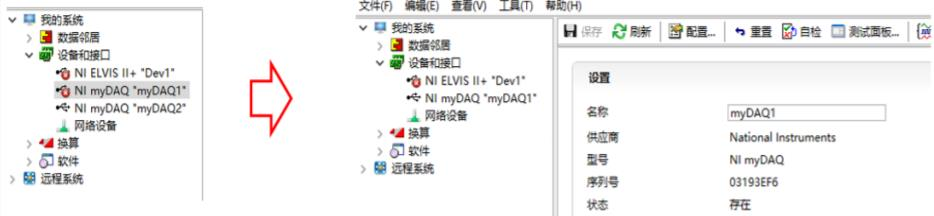
\includegraphics[width=\textwidth]{3-1.png}
    \end{figure} 
    \newpage
	\item 角度零点校正:转动电机指向 0°位置,双击桌面的“玻尔机械混沌摆”启动程序后,软件会实时显示摆轮角度,
    用手拨动摆轮,使白色箭头从负 140°至正 140°摆动一次,然后使箭头对准 0°。此时观察软件实时显示的摆轮
    角度是否正确。如不正确,需在“零点校正”中输入符号相反的数值,之后再次转动摆轮检查角度显示是否正确。({\color{red}注:每次启动程序,都需要进行角度校正。如果在程序运行过程中,中途点击过“角度采集”按钮,“零度校
    正”一般不需要重新设置,只需手动让摆轮从左到右大幅摆动一次,角度显示即可恢复正常。})
	\item 安装重物后,转动电机指向 0°位置,调节重物离转轴的距离,使摆轮偏转后稳定在 35~50°之间。
    4.用于电机供电的电源,电压设置为 15V;点击“电机开关”,电机才会启动;点击“设置频率”,电机频率才会
    更新。(注:用于电机供电的电源打开时,转动电机时的阻力会增大)
    \item 数据保存:{\color{red}软件保存的数据都是保存时刻前 240 秒的数据。}软件在“保存间隔”和“稳定时间”均会自动保存一
    次数据,可以根据“已用时间”和文件名进行区分(也可以设置“保存间隔”和“稳定时间”相等,这样软件在达到
    “稳定时间”时保留一次数据)。点击“保存数据”,软件会即刻保存数据一次。
    
\end{enumerate}}

\clearpage
\tableofcontents
\clearpage

\setcounter{section}{0}
\section{实验BD1\ 复摆与混沌}
	
\subsection{实验目的}
\begin{enumerate}
	\item 观察复摆的振动现象,学习复摆的运动方程;
	\item 了解混沌的基本特征,理解非线性方程解的稳定性与混沌的关系;
	\item 设置不同的参数,测量角度时序图、相图、功率谱、探索产生混沌的条件;
	\item 熟悉基于LabVIEW 对实验过程进行控制及数据处理。
\end{enumerate}

\subsection{仪器用具}
\begin{table}[htbp]
	\centering
	\renewcommand\arraystretch{1.6}
	% \setlength{\tabcolsep}{10mm}
	\begin{tabular}{p{0.05\textwidth}|p{0.20\textwidth}|p{0.05\textwidth}|p{0.5\textwidth}}
	\hline
	编号& 仪器用具名称 & 数量 &  主要参数(型号,测量范围,测量精度等) \\
	\hline
	1&玻尔振动混沌实验仪&1 &COC-JCHD\\
	\hline
	2&myDAQ  &1&\\
	\hline
	3&直流电源 & 1 &RXN-1502D \\
	\hline
	4&物理天平&1 &  \\
	\hline
	5& 钢尺&1& \\
	\hline
\end{tabular}
\end{table}

\subsection{实验前思考题}
\begin{question}
	混沌的基本特征是什么?如何认定一个系统进入了混沌状态??
	\tcblower
	混沌的基本特征是非周期性、不确定性、不可重复、不可预测,尤其是输出状态对初始条
件的敏感依赖性。

    当一个系统的相图的曲线长时间不能闭合,曲线轨迹看似随机无规律,便可认为系统进入
了混沌态。
\end{question}

\begin{question}
	请求出方程$\frac{\d ^2\theta}{\d t^2}+\frac{r}{I+md^2}\frac{\d \theta}{\d t}-\frac{mgd-c}{I+md^2}\theta+\frac{mgd}{6(I+md^2)}\theta^3=\frac{M_0}{I+md^2}\cos\omega t$
    的稳定解$\theta_0$并推导出方程$\frac{\d ^2 x}{\d \tau^2}+\mu\frac{\d x}{\d\tau}-x+x^3=\eta\cos\Omega\tau$
	\tcblower
	当$\frac{M_0}{I+md^2}\to 0,\frac{\d^2\theta}{\d t^2}\to 0,\frac{\d \theta}{\d t}\to 0$,有
    \[\frac{mgd-c}{I+md^2}\theta=\frac{mgd}{6(I+md^2)}\theta^3\]
    当$mgd>c$时:

    可解得$\theta_1=0,\theta_2=-\sqrt{6(1-\frac{c}{mgd})},\theta_3=\sqrt{6(1-\frac{c}{mgd})}$
    现不认为$\frac{\d ^2\theta}{\d t^2}=0$,将带有微扰的$\theta=\theta_2+\delta\theta$代入可得
    $\ddot{\theta}=\frac{-mgd}{6(I+md^2)}(\theta_2+\delta\theta)\delta\theta(\theta_2-\theta_3+\delta\theta)$
    由此得$\frac{\ddot{\theta}}{\delta\theta}<0$,加速度为负反馈故$\theta_2$为稳定解。同理,$\theta_3$也是稳定解。
    
    将$\theta=\theta_1+\delta\theta$代入,得$\ddot{\theta}=\frac{-mgd}{6(I+md^2)}\delta\theta(\delta\theta-\theta_2)(\delta\theta-\theta_3)\to \frac{\ddot{\theta}}{\delta\theta}>0$,
    故$\theta_1$不是稳定解。

	当$mgd<c$时方程仅有一平衡解$\theta=0$,为稳定解。
	
	令$x=\frac{\theta}{\theta_3}$,则方程变为
	\[\frac{\sqrt{6}}{\sqrt{mgd}}\sqrt{mgd-c}(\frac{\d^2 x}{\d t^2}+\frac{r}{I+md^2}\frac{\d x}{\d t})+\frac{\sqrt{6}(mgd-c)^{\frac{3}{2}}}{(I+md^2)\sqrt{mgd}}(x^3-x)=\frac{M_0}{I+md^2}\cos\omega t\]
	设$\tau=t\sqrt{\frac{mgd-c}{I+md^2}}$,则方程变为
	\[\frac{\sqrt{6}(mgd-c)^{\frac{3}{2}}}{\sqrt{mgd}}(\frac{\d^2x}{\d \tau^2}+\frac{r}{\sqrt{mgd-c}\sqrt{I+md^2}}\frac{\d x}{\d\tau})+\frac{\sqrt{6}(mgd-c)^{\frac{3}{2}}}{\sqrt{mgd}}(x^3-x)=M_0\cos\frac{\omega\sqrt{I+md^2}}{\sqrt{mgd-c}} \tau\]
	即
	\[\frac{\d^2x}{\d\tau^2}+{\color{red}\frac{r}{\sqrt{mgd-c}\sqrt{I+md^2}}}\frac{\d x}{\d\tau}+x^3-x={\color{red}\frac{M_0\sqrt{mgd}}{\sqrt{6}(mgd-c)^{\frac{3}{2}}}}\cos{\color{red}\frac{\omega\sqrt{I+md^2}}{\sqrt{mgd-c}}} \tau\]
\end{question}

\begin{question}
	自编计算机程序或根据附录一提供的模拟程序,设置几组不同的参数,模拟摆轮的角度时序图、相图、功率谱,
	探索产生混沌现象的条件。
	\tcblower
	\textbf{【第一组模拟】}
	我们固定$\mu = 0.75$, $\eta = 1$, $T = 300$, $x(0) = 0$, $x'(0) = 1$,调整$\Omega:0.70 \to 0.875$,得到下
	面一系列图像。生成\ref{1}及下列图像的代码示例见附录。
	\begin{figure}[H]
		\centering  %图片全局居中
		\subfloat[$\Omega=0.70$]{
		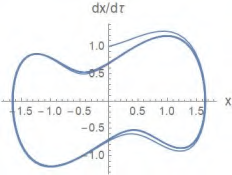
\includegraphics[width=0.25\textwidth]{3-2.png}}
		\subfloat[$\Omega=0.75$]{	
		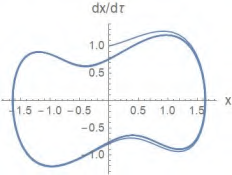
\includegraphics[width=0.25\textwidth]{3-3.png}}
		\subfloat[$\Omega=0.80$]{
		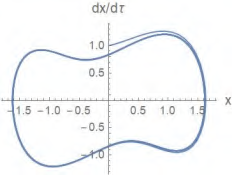
\includegraphics[width=0.25\textwidth]{3-4.png}}
		\subfloat[$\Omega=0.85$]{
		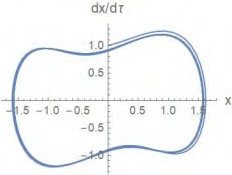
\includegraphics[width=0.25\textwidth]{3-5.png}}
		\label{1}
		\caption{系统显周期性时的一些相图}
	\end{figure}
	\begin{figure}[H]     
		\centering  %图片全局居中     
		\subfloat[角度时序图]{     
			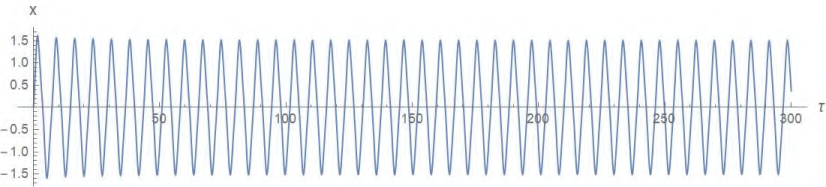
\includegraphics[width=\textwidth]{3-6.png}}   
			
		\subfloat[相图]{         
			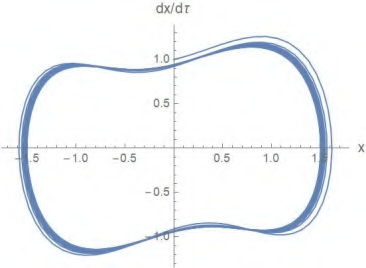
\includegraphics[width=0.5\textwidth]{3-7.png}}     
		\subfloat[功率谱]{     
			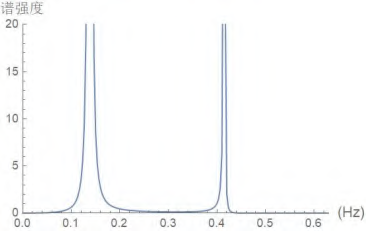
\includegraphics[width=0.5\textwidth]{3-8.png}}     
		\caption{$\Omega=0.869$}     
	\end{figure}  
	\begin{figure}[H]     
		\centering  %图片全局居中     
		\subfloat[角度时序图]{     
			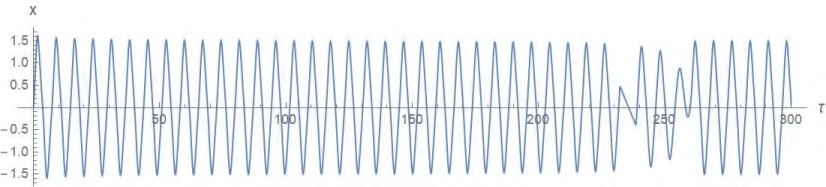
\includegraphics[width=\textwidth]{3-9.png}}  

		\subfloat[相图]{         
			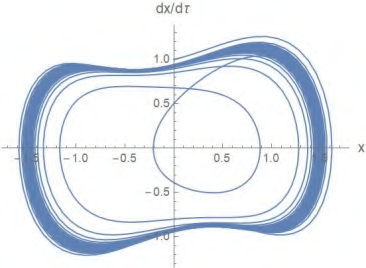
\includegraphics[width=0.5\textwidth]{3-10.png}}     
		\subfloat[功率谱]{     
			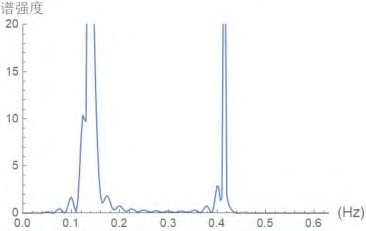
\includegraphics[width=0.5\textwidth]{3-11.png}}     
		\caption{$\Omega=0.870$}     
	\end{figure}  
	
	\begin{figure}[H]     
		\centering  %图片全局居中     
		\subfloat[角度时序图]{     
			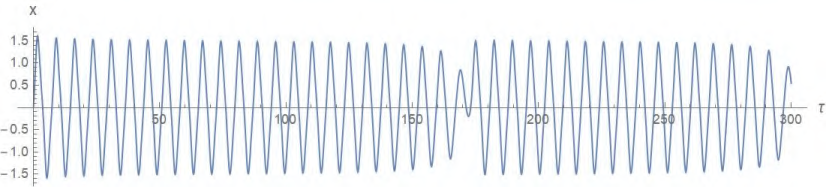
\includegraphics[width=\textwidth]{3-12.png}}  

		\subfloat[相图]{         
			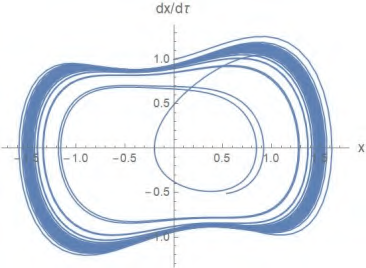
\includegraphics[width=0.5\textwidth]{3-13.png}}     
		\subfloat[功率谱]{     
			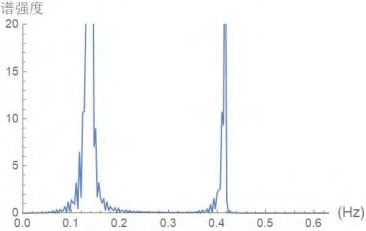
\includegraphics[width=0.5\textwidth]{3-14.png}}     
		\caption{$\Omega=0.871$}     
	\end{figure}  
	
	\begin{figure}[H]     
		\centering  %图片全局居中     
		\subfloat[角度时序图]{     
			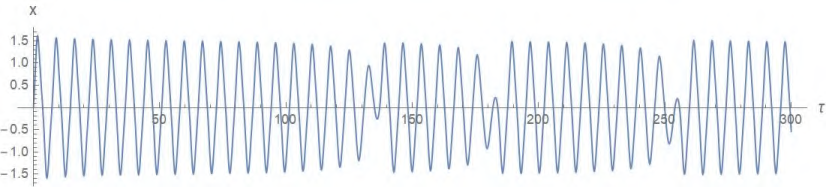
\includegraphics[width=\textwidth]{3-15.png}}

		\subfloat[相图]{         
			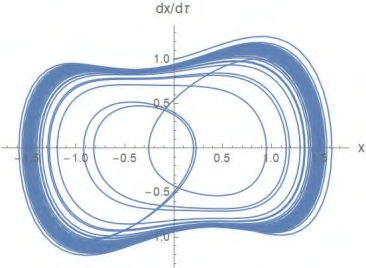
\includegraphics[width=0.5\textwidth]{3-16.png}}     
		\subfloat[功率谱]{     
			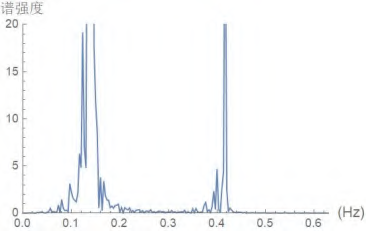
\includegraphics[width=0.5\textwidth]{3-17.png}}     
		\caption{$\Omega=0.872$}     
	\end{figure}  
	
	\begin{figure}[H]     
		\centering  %图片全局居中     
		\subfloat[角度时序图]{     
			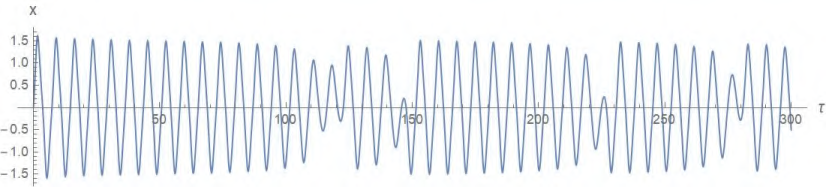
\includegraphics[width=\textwidth]{3-18.png}}

		\subfloat[相图]{         
			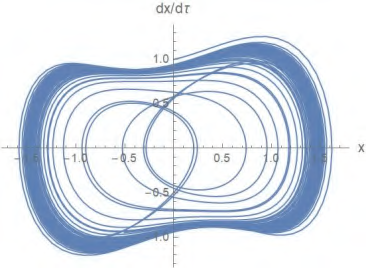
\includegraphics[width=0.5\textwidth]{3-19.png}}     
		\subfloat[功率谱]{     
			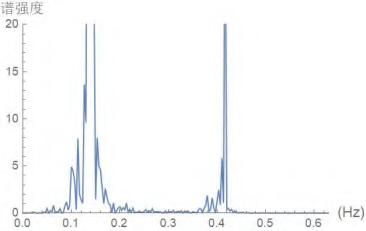
\includegraphics[width=0.5\textwidth]{3-20.png}}     
		\caption{$\Omega=0.873$}     
	\end{figure}  
	
	\begin{figure}[H]     
		\centering  %图片全局居中     
		\subfloat[角度时序图]{     
			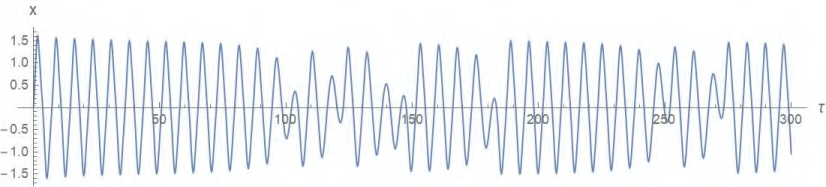
\includegraphics[width=\textwidth]{3-21.png}}

		\subfloat[相图]{         
			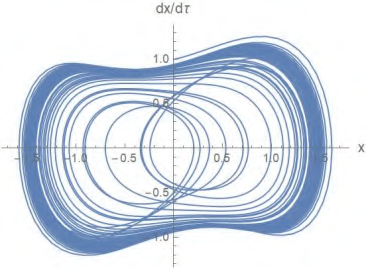
\includegraphics[width=0.5\textwidth]{3-22.png}}     
		\subfloat[功率谱]{     
			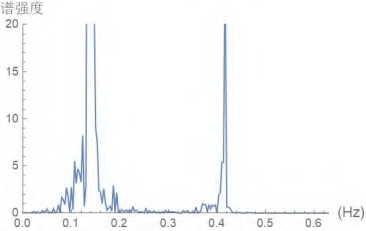
\includegraphics[width=0.5\textwidth]{3-23.png}}     
		\caption{$\Omega=0.874$}     
	\end{figure}
	
	\begin{figure}[H]     
		\centering  %图片全局居中     
		\subfloat[角度时序图]{     
			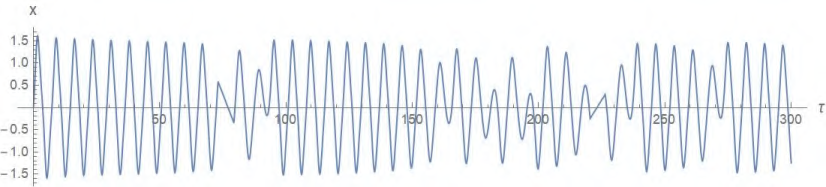
\includegraphics[width=\textwidth]{3-24.png}} 

		\subfloat[相图]{         
			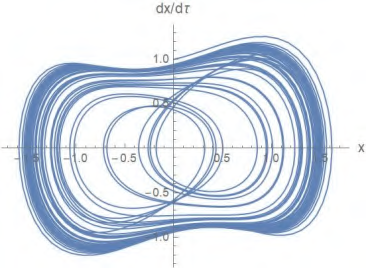
\includegraphics[width=0.5\textwidth]{3-25.png}}     
		\subfloat[功率谱]{     
			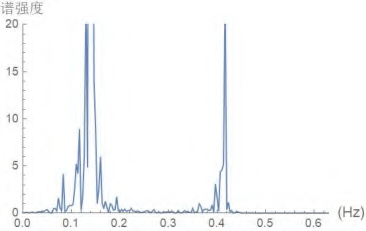
\includegraphics[width=0.5\textwidth]{3-26.png}}     
		\caption{$\Omega=0.875$}     
	\end{figure} 
	我们发现,“平衡周期”可以“稳定”,即这条闭合轨迹附近的初始条件会在相图中收敛于
这条闭合轨迹;也可以“不稳定”,即这条闭合轨迹附近的初始条件会首先在相图中沿着这条闭
合轨迹附近运行一段时间,然后脱离这条轨迹,走向混沌(或其他平衡周期)。{\color{red}由此可见,当一
个比较简单的“稳定平衡周期”随参数变化为“不稳定平衡周期”,本来应该落入“稳定平衡周
期”的初始条件可能产生混沌。其中,混沌发生所需的时间(角度时序图明显失去周期性)也
会渐渐变短,如果模拟的时间不够长,那就并不能明确界定“周期”与“混沌”。 }

\textbf{【第二组模拟】}
再固定$\mu=0.6$,$\eta=1$,$T=300$,$x(0)=1$,$x'(0)=1$,调整$\Omega:1.70112\to 1.70116$,得到下面一系列图像:
\begin{figure}[H]     
	\centering  %图片全局居中     
	\subfloat[角度时序图]{     
		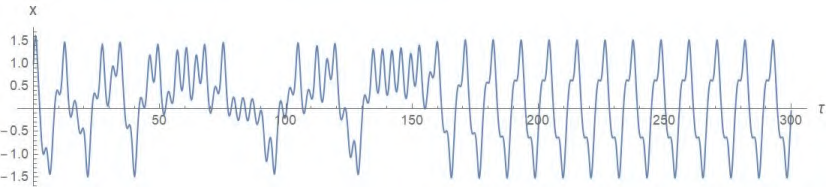
\includegraphics[width=\textwidth]{3-27.png}} 

	\subfloat[相图]{         
		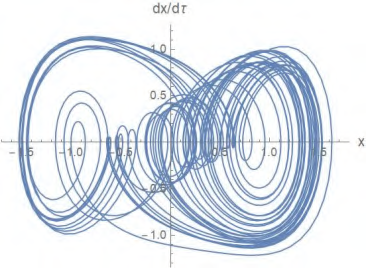
\includegraphics[width=0.5\textwidth]{3-28.png}}     
	\subfloat[功率谱]{     
		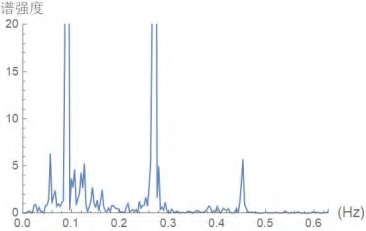
\includegraphics[width=0.5\textwidth]{3-29.png}}     
	\caption{$\Omega=1.70112$}     
\end{figure}
\begin{figure}[H]     
	\centering  %图片全局居中     
	\subfloat[角度时序图]{     
		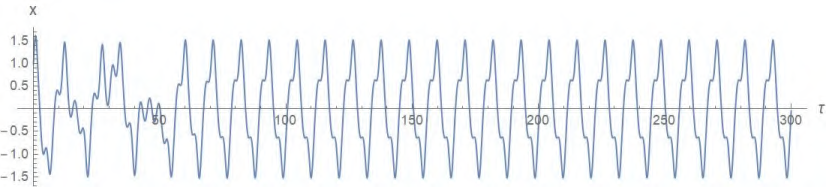
\includegraphics[width=\textwidth]{3-30.png}} 

	\subfloat[相图]{         
		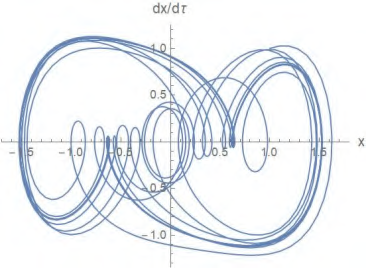
\includegraphics[width=0.5\textwidth]{3-31.png}}     
	\subfloat[功率谱]{     
		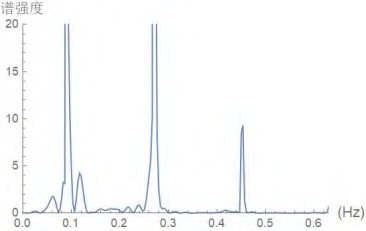
\includegraphics[width=0.5\textwidth]{3-32.png}}     
	\caption{$\Omega=1.70113$}     
\end{figure}
\begin{figure}[H]     
	\centering  %图片全局居中     
	\subfloat[角度时序图]{     
		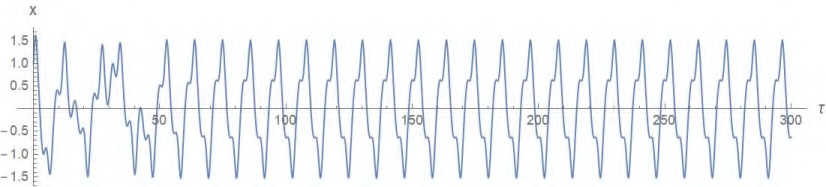
\includegraphics[width=\textwidth]{3-33.png}} 

	\subfloat[相图]{         
		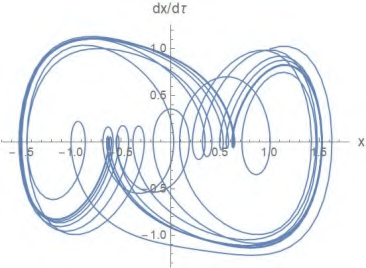
\includegraphics[width=0.5\textwidth]{3-34.png}}     
	\subfloat[功率谱]{     
		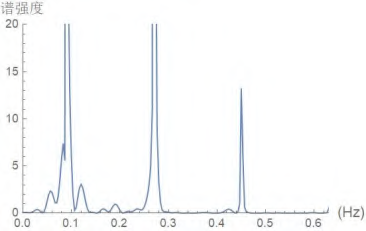
\includegraphics[width=0.5\textwidth]{3-35.png}}     
	\caption{$\Omega=1.70114$}     
\end{figure}
\begin{figure}[H]     
	\centering  %图片全局居中     
	\subfloat[角度时序图]{     
		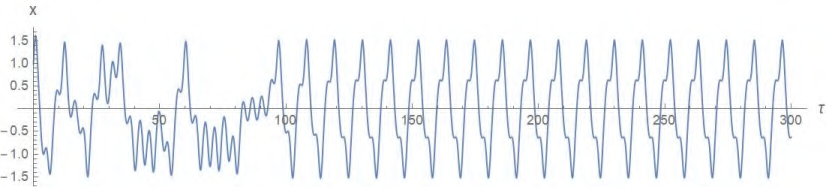
\includegraphics[width=\textwidth]{3-39.png}} 

	\subfloat[相图]{         
		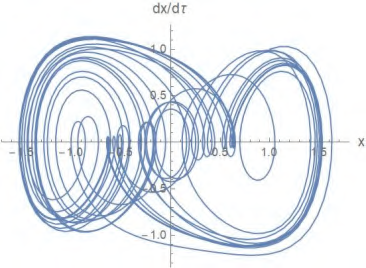
\includegraphics[width=0.5\textwidth]{3-40.png}}     
	\subfloat[功率谱]{     
		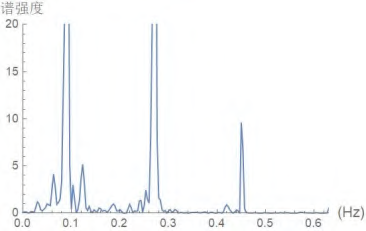
\includegraphics[width=0.5\textwidth]{3-41.png}}     
	\caption{$\Omega=1.70116$}     
\end{figure}

\textbf{【第三组模拟】}
再固定$\mu=0.6$,$\eta=1$,$T=300$,$\Omega=1.70116$,$x'(0)=1$调整$x(0):1.0000\to 1.0003$得到下列一系列图像
\begin{figure}[H]     
	\centering  %图片全局居中     
	\subfloat[角度时序图]{     
		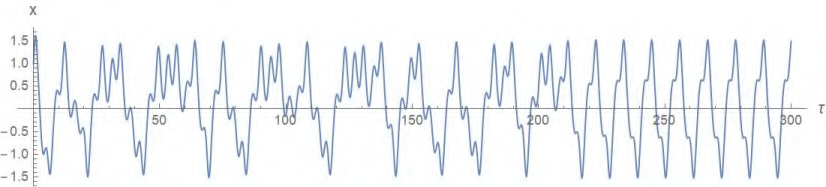
\includegraphics[width=\textwidth]{3-42.png}} 

	\subfloat[相图]{         
		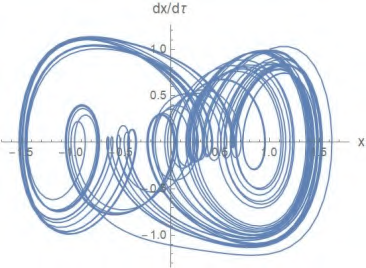
\includegraphics[width=0.5\textwidth]{3-43.png}}     
	\subfloat[功率谱]{     
		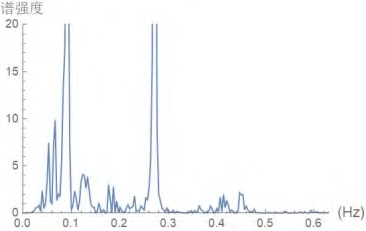
\includegraphics[width=0.5\textwidth]{3-44.png}}     
	\caption{$x(0)=1.0001$}     
\end{figure}

\begin{figure}[H]     
	\centering  %图片全局居中     
	\subfloat[角度时序图]{     
		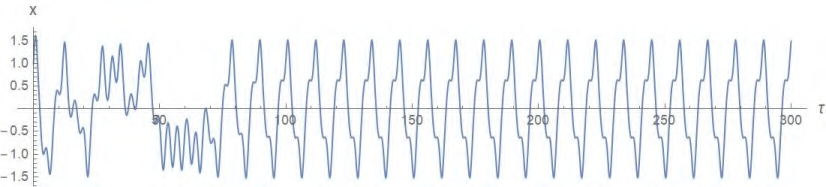
\includegraphics[width=\textwidth]{3-45.png}} 

	\subfloat[相图]{         
		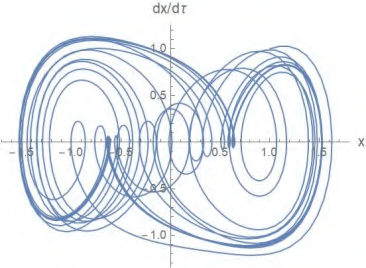
\includegraphics[width=0.5\textwidth]{3-46.png}}     
	\subfloat[功率谱]{     
		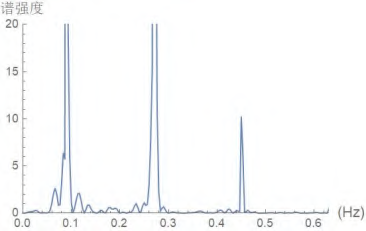
\includegraphics[width=0.5\textwidth]{3-47.png}}     
	\caption{$x(0)=1.0002$}     
\end{figure}

\begin{figure}[H]     
	\centering  %图片全局居中     
	\subfloat[角度时序图]{     
		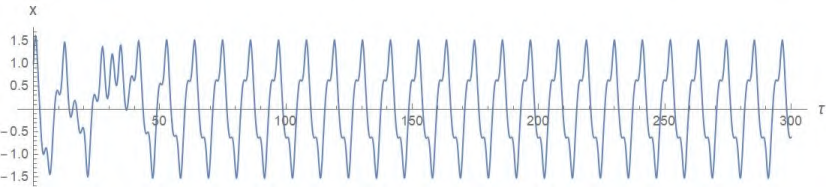
\includegraphics[width=\textwidth]{3-48.png}} 

	\subfloat[相图]{         
		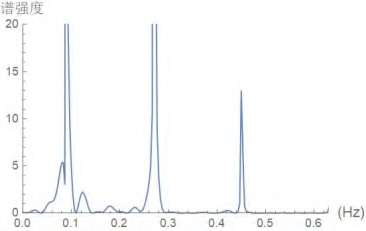
\includegraphics[width=0.5\textwidth]{3-49.png}}     
	\subfloat[功率谱]{     
		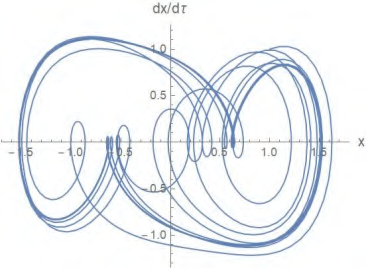
\includegraphics[width=0.5\textwidth]{3-50.png}}     
	\caption{$x(0)=1.0003$}     
\end{figure}
{\color{red}由此可见,一个比较复杂的“稳定平衡周期”在接近“不稳定”时,从初始到稳定所需时
间非常难以估计。如果模拟的时间不够长,可能将“周期”误判为“混沌”。

综上所述,初始条件无法靠近或无“稳定平衡周期”可以产生混沌。若将“一定时间内(如
2 分钟、2 小时等)无明显周期”也视为混沌,那么“稳定平衡周期”的收敛速度过慢也可以造
成一定时间内的混沌。}
\end{question}

\begin{question}
	在振动不稳定区域,选取两个不同的初始值,利用计算机模拟并比较系统的振动状态
	\tcblower
	固定$\mu=0.6$,$\eta=1$,$T=300$,$\Omega=1.76$,$x'(0)=1$调整$x(0):0.0000\to 0.0001$得到下列一系列图像
	\begin{figure}[H]     
		\centering  %图片全局居中     
		\subfloat[角度时序图]{     
			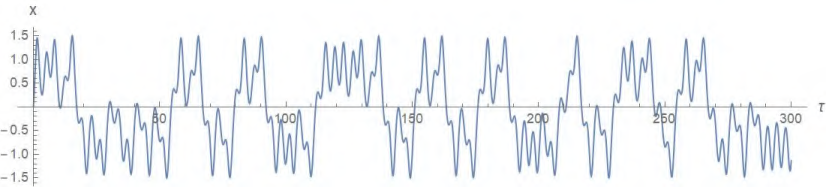
\includegraphics[width=\textwidth]{3-51.png}} 
	
		\subfloat[相图]{         
			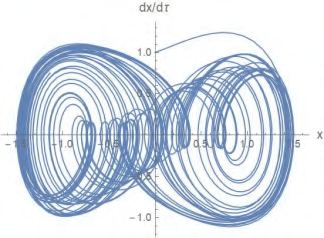
\includegraphics[width=0.5\textwidth]{3-52.png}}     
		\subfloat[功率谱]{     
			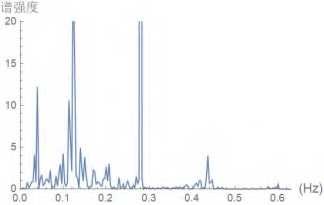
\includegraphics[width=0.5\textwidth]{3-53.png}}     
		\caption{$x(0)=0.0000$}     
	\end{figure}

	\begin{figure}[H]     
		\centering  %图片全局居中     
		\subfloat[角度时序图]{     
			\includegraphics[width=\textwidth]{3-54.png}} 
	
		\subfloat[相图]{         
			\includegraphics[width=0.5\textwidth]{3-55.png}}     
		\subfloat[功率谱]{     
			\includegraphics[width=0.5\textwidth]{3-56.png}}     
		\caption{$x(0)=0.0001$}     
	\end{figure}
	两组参数中,$x(0)$ 仅相差$10^{−4}$,但角度时序图在$t = 50$s 之后已经完全不同,$t = 0 - 300$s
中的频谱也差别非常大,这个现象可以验证混沌对初始条件的敏感依赖性。
\end{question}


\clearpage
\setLhead{中山大学物理与天文学院基础物理实验记录}
\begin{table}
	\renewcommand\arraystretch{1.7}
	\centering
	\begin{tabularx}{\textwidth}{|X|X|X|X|}
	\hline
	专业:& 物理学类 &年级:& 2023级 \\
	\hline
	姓名:& 姚昊廷 &学号:&22322091  \\
	\hline
	室温:&24.5$^\circ$C&实验地点:&A507\ D4\\
	\hline
	学生签名:& & 评分: &\\
	\hline
	实验时间:& 2024.10.10& 教师签名:&\\
	\hline
	\end{tabularx}
\end{table}

\section{实验BD1\ 复摆与混沌}
\textbf{分析与讨论}

1.阻尼振动、受迫振动
\begin{figure}[H]
	\includegraphics[width=\textwidth]{姚昊廷22322091/140阻尼.jpg}
	\caption{初始角度140°时的阻尼振动相图}
\end{figure}
\begin{figure}[H]
	\includegraphics[width=\textwidth]{3-57.png}
	\caption{驱动电压15V,电机频率0.5Hz的受迫振动开始时相图}
\end{figure}

\begin{figure}[H]
	\includegraphics[width=\textwidth]{姚昊廷22322091/15V受迫.jpg}
	\caption{驱动电压15V,电机频率0.5Hz的受迫振动稳定时相图}
\end{figure}

2.增加重物的混沌摆

重物质量:46.97g

重物距中心距离:29.50mm
\begin{figure}[H]
	\includegraphics[width=\textwidth]{姚昊廷22322091/0.3Hz加重物.jpg}
	\caption{0.3Hz}
\end{figure}

\begin{figure}[H]
	\includegraphics[width=\textwidth]{姚昊廷22322091/0.375Hz加重物.jpg}
	\caption{0.375Hz}
\end{figure}

\begin{figure}[H]
	\includegraphics[width=\textwidth]{姚昊廷22322091/0.45Hz加重物.jpg}
	\caption{0.45Hz}
\end{figure}

\begin{figure}[H]
	\includegraphics[width=\textwidth]{姚昊廷22322091/0.525Hz加重物.jpg}
	\caption{0.525Hz}
\end{figure}

\begin{figure}[H]
	\includegraphics[width=\textwidth]{姚昊廷22322091/0.3Hz加重物.jpg}
	\caption{0.6Hz}
\end{figure}

3.改变摆轮初始角度下摆轮运动状态
\begin{figure}[H]
	\includegraphics[width=\textwidth]{姚昊廷22322091/0.275Hz8.856.jpg}
	\caption{0.275Hz初始摆角8.856}
\end{figure}

\begin{figure}[H]
	\includegraphics[width=\textwidth]{姚昊廷22322091/0.275Hz-130.jpg}
	\caption{0.275Hz初始摆角-130}
\end{figure}
\subsection{实验过程中遇到的问题记录}



\clearpage
\setLhead{中山大学物理与天文学院基础物理实验分析与讨论}
\begin{table}
	\renewcommand\arraystretch{1.7}
	\begin{tabularx}{\textwidth}{|X|X|X|X|}
	\hline
	专业:& 物理学 &年级:& 2023级\\
	\hline
	姓名: &姚昊廷 & 学号:& 22322091\\
	\hline
    日期:&2024.10.10 & 评分: &\\
	\hline
	\end{tabularx}
\end{table}

\section{实验BD1\ 复摆与混沌}
\textbf{【分析与讨论】}

根据中山大学物理与天文学院基础物理实验记录所得到的数据与结果图进行分析讨论。

1. 阻尼振动、受迫振动(结合实验记录数据及图片分析每次实验的特征

阻尼振动:阻尼振动中,非保守力的力矩只有与角速度相反方向的确定大小的阻尼,所以对于速度相
空间里的每个点,都可以对应一个矢量,这个矢量表示系统在这个点时,系统在速度相空间的
广义速度。这些矢量构成了速度相空间里的一个矢量场,如果将“相邻的首尾相接的”矢量相
连,可以得到一个“风速图”(不过是有源场),可以猜测,风速图呈螺旋收缩状。粒子在这个“风
速图”中的初始位置可以唯一确定粒子的轨迹,即系统的初始条件可以唯一确定系统演化(演
化与绝对时间无关)。更直观的是,由于阻尼造成的机械能损失,使得系统没有周期性,所以系
统在速度相空间的轨迹不会与自身相交。这与我们实际测到的相图基本相符。
另外,我们可以推测相图中轨迹上角速度为零的点为角度的极值点(或驻点),但与我们测
到的相图有所偏差。我们只能认为这是软件计算角速度的算法造成的偏差。

受迫振动:初始条件为“角度和角速度均为零”的受迫振动在第十个周期左右已经区域稳定。收敛过
程中,振动幅度先是增大到大于稳定值,再重新缩小,有一定的振荡,但收敛已经非常迅速。由
此可以验证方程
$$I\ddot{\theta}+r\dot{\theta}-c\theta=M_0\cos\omega t$$
的解的稳定性。

2.增加重物的混沌摆

增加重物的混沌摆中,当其他参数都调整至实验中的值并固定,然后缓慢改
变$\omega$时,系统的周期/混沌状态会随之慢慢改变。总体来说,当$\omega$从0.6Hz 下降到0.3Hz 的过
程中,周期逐渐复杂化,周期的稳定性渐渐变差(能承受的最大微扰变小),逐渐变得混沌,但未能测出(如果理论值存在)“周期”与“混沌”
的临界频率(我们的测量结果大致在0.3 ∼ 0.325Hz 之间)。

3.改变摆轮初始角度下摆轮运动状态w

我们对0.275Hz的受迫振动选取-130和8.856两组初始条件,最后演化趋于混沌的两支。

\textbf{【实验思考题】}

1.比较玻尔振动仪的动力学方程与混沌实验仪的动力学方程,叙述它们的物理意义以及产生混沌的条件。

玻尔振动仪的动力学方程为:
$$I\ddot{\theta}+r\dot{\theta}-c\theta=M_0\cos\omega t$$
其中$I$为摆轮对转轴的转动惯量,$\theta$为摆轮的扭转角,$c$ 为扭转恢复力系数,$r$ 为阻力矩系数
混沌实验仪的动力学方程为:
$$(I+md^2)\ddot{\theta}+r\dot{\theta}-c\theta-mgd\sin\theta=M_0\cos\omega t$$
取近似后有
$$(I+{\color{red}md^2})\ddot{\theta}+r\dot{\theta}-(c{\color{red}-mgd})\theta{\color{red}+\frac{mgd}{6}\theta^3}=M_0\cos\omega t$$
其中标红部分为加重物后新出现的项,$md^2$ 为重物关于转轴的转动惯量,$mgd \sin \theta$ 为重物
重力对系统的力矩。
产生混沌的条件为混沌实验仪器的频率明显低于“固有频率”,且有恰当的初始条件。可
能还需要$c$,$ md^2$, $mgd$, $M_0$ 的比例在一定的合适范围内。

2、比较分析不加重物时的相图与加重物后混沌摆的相图,理解用相图分析非线性运动规律的优越性。

相图将系统表示在相空间中,可以表示系统的位形和广义速度。相图可以将周期的波形画
成闭合曲线,直观显示“周期”与“周期”的稳定性。相空间中可以将吸引子直观地表示在(±θ0, 0)
的位置,可以将比较长时间的系统状态的轨迹汇集在一张不会很长的图中,同时显示出时序图
中难以表现的“广义速度”,也略去了“具体时间”和“运动周期”的相对不重要的物理量。


\clearpage
% ---------------------------------------------------------------------
%   参考文献
%   注:使用参考文献时应按照xelatex->bibtex->xelatex->xelatex顺序进行编译
\phantomsection
%\addcontentsline{toc}{section}{参考文献}
\bibliographystyle{unsrt}
\bibliography{myref}
%\begin{thebibliography}{9}
	%\bibitem{ref1} 凤飞龙,黄育红,金蔚,王公正,崔致远,“外推法计算冰的熔解热的理论依据及Matlab实现方案”,《大学物理》,第42卷,第2期
%\end{thebibliography}


\clearpage
\appendix
\appendixpage
\addappheadtotoc
\subsection*{相图代码}
\includepdf[pages=-]{chaos.pdf}
\subsection*{原件扫描}
\includepdf[pages=-]{实验3原件.pdf}

\subsection*{桌面}
\begin{figure}[!h]
	\includegraphics[width=0.95\textwidth]{实验3桌面.jpg}
\end{figure}
\end{document}
%杀杀杀杀杀杀杀杀杀杀杀杀杀杀杀杀杀杀杀杀杀杀杀杀杀杀杀杀杀杀杀杀杀杀杀杀杀杀杀杀杀杀杀杀杀杀杀杀杀杀杀杀杀杀杀杀杀杀杀杀杀杀杀杀杀杀杀杀杀杀杀杀杀杀杀杀杀杀
%杀杀杀杀杀杀杀杀杀杀杀杀杀杀杀杀杀杀杀杀杀杀杀杀杀杀杀杀杀杀杀杀杀杀杀杀杀杀杀杀杀杀杀杀杀杀杀杀杀杀杀杀杀杀杀杀杀杀杀杀杀杀杀杀杀杀杀杀杀杀杀杀杀杀 杀杀杀杀杀杀杀杀杀杀杀杀杀杀杀杀杀杀杀杀杀杀杀杀杀杀杀杀杀杀杀杀杀杀杀杀杀杀杀杀杀杀杀杀杀杀杀杀杀杀杀杀杀杀杀杀杀杀杀杀杀杀杀杀杀杀杀杀杀杀杀杀杀杀 杀杀杀杀杀杀杀杀杀杀杀杀杀杀杀杀杀杀杀杀杀杀杀杀杀杀杀杀杀杀杀杀杀杀杀杀杀杀杀杀杀杀杀杀杀杀杀杀杀杀杀杀杀杀杀杀杀杀杀杀杀杀杀杀杀杀杀杀杀杀杀杀杀杀
%杀杀杀杀杀杀杀杀杀杀杀杀杀杀杀杀杀杀杀杀杀杀杀杀杀杀杀杀杀杀杀杀杀杀杀杀杀杀杀杀杀杀杀杀杀杀杀杀杀杀杀杀杀杀杀杀杀杀杀杀杀杀杀杀杀杀杀杀杀杀杀杀杀杀 杀杀杀杀杀杀杀杀杀杀杀杀杀杀杀杀杀杀杀杀杀杀杀杀杀杀杀杀杀杀杀杀杀杀杀杀杀杀杀杀杀杀杀杀杀杀杀杀杀杀杀杀杀杀杀杀杀杀杀杀杀杀杀杀杀杀杀杀杀杀杀杀杀杀
%杀杀杀杀杀杀杀杀杀杀杀杀杀杀杀杀杀杀杀杀杀杀杀杀杀杀杀杀杀杀杀杀杀杀杀杀杀杀杀杀杀杀杀杀杀杀杀杀杀杀杀杀杀杀杀杀杀杀杀杀杀杀杀杀杀杀杀杀杀杀杀杀杀杀 杀杀杀杀杀杀杀杀杀杀杀杀杀杀杀杀杀杀杀杀杀杀杀杀杀杀杀杀杀杀杀杀杀杀杀杀杀杀杀杀杀杀杀杀杀杀杀杀杀杀杀杀杀杀杀杀杀杀杀杀杀杀杀杀杀杀杀杀杀杀杀杀杀杀杀杀杀杀杀杀杀杀杀杀杀杀杀杀杀杀杀杀杀杀杀杀杀杀杀杀杀杀杀杀杀杀杀杀杀杀杀杀杀杀杀杀杀杀杀杀杀杀杀杀杀杀杀杀杀杀杀杀杀杀
%杀杀杀杀杀杀杀杀杀杀杀杀杀杀杀杀杀杀杀杀杀杀杀杀杀杀杀杀杀杀杀杀杀杀杀杀杀杀杀杀杀杀杀杀杀杀杀杀杀杀杀杀杀杀杀杀杀杀杀杀杀杀杀杀杀杀杀杀杀杀杀杀杀杀 杀杀杀杀杀杀杀杀杀杀杀杀杀杀杀杀杀杀杀杀杀杀杀杀杀杀杀杀杀杀杀杀杀杀杀杀杀杀杀杀杀杀杀杀杀杀杀杀杀杀杀杀杀杀杀杀杀杀杀杀杀杀杀杀杀杀杀杀杀杀杀杀杀杀 杀杀杀杀杀杀杀杀杀杀杀杀杀杀杀杀杀杀杀杀杀杀杀杀杀杀杀杀杀杀杀杀杀杀杀杀杀杀杀杀杀杀杀杀杀杀杀杀杀杀杀杀杀杀杀杀杀杀杀杀杀杀杀杀杀杀杀杀杀杀杀杀杀杀
%杀杀杀杀杀杀杀杀杀杀杀杀杀杀杀杀杀杀杀杀杀杀杀杀杀杀杀杀杀杀杀杀杀杀杀杀杀杀杀杀杀杀杀杀杀杀杀杀杀杀杀杀杀杀杀杀杀杀杀杀杀杀杀杀杀杀杀杀杀杀杀杀杀杀 杀杀杀杀杀杀杀杀杀杀杀杀杀杀杀杀杀杀杀杀杀杀杀杀杀杀杀杀杀杀杀杀杀杀杀杀杀杀杀杀杀杀杀杀杀杀杀杀杀杀杀杀杀杀杀杀杀杀杀杀杀杀杀杀杀杀杀杀杀杀杀杀杀杀
%杀杀杀杀杀杀杀杀杀杀杀杀杀杀杀杀杀杀杀杀杀杀杀杀杀杀杀杀杀杀杀杀杀杀杀杀杀杀杀杀杀杀杀杀杀杀杀杀杀杀杀杀杀杀杀杀杀杀杀杀杀杀杀杀杀杀杀杀杀杀杀杀杀杀 杀杀杀杀杀杀杀杀杀杀杀杀杀杀杀杀杀杀杀杀杀杀杀杀杀杀杀杀杀杀杀杀杀杀杀杀杀杀杀杀杀杀杀杀杀杀杀杀杀杀杀杀杀杀杀杀杀杀杀杀杀杀杀杀杀杀杀杀杀杀杀杀杀杀杀杀杀杀杀杀杀杀杀杀杀杀杀杀杀杀杀杀杀杀杀杀杀杀杀杀杀杀杀杀杀杀杀杀杀杀杀杀杀杀杀杀杀杀杀杀杀杀杀杀杀杀杀杀杀杀杀杀杀杀
%杀杀杀杀杀杀杀杀杀杀杀杀杀杀杀杀杀杀杀杀杀杀杀杀杀杀杀杀杀杀杀杀杀杀杀杀杀杀杀杀杀杀杀杀杀杀杀杀杀杀杀杀杀杀杀杀杀杀杀杀杀杀杀杀杀杀杀杀杀杀杀杀杀杀 杀杀杀杀杀杀杀杀杀杀杀杀杀杀杀杀杀杀杀杀杀杀杀杀杀杀杀杀杀杀杀杀杀杀杀杀杀杀杀杀杀杀杀杀杀杀杀杀杀杀杀杀杀杀杀杀杀杀杀杀杀杀杀杀杀杀杀杀杀杀杀杀杀杀 杀杀杀杀杀杀杀杀杀杀杀杀杀杀杀杀杀杀杀杀杀杀杀杀杀杀杀杀杀杀杀杀杀杀杀杀杀杀杀杀杀杀杀杀杀杀杀杀杀杀杀杀杀杀杀杀杀杀杀杀杀杀杀杀杀杀杀杀杀杀杀杀杀杀
%杀杀杀杀杀杀杀杀杀杀杀杀杀杀杀杀杀杀杀杀杀杀杀杀杀杀杀杀杀杀杀杀杀杀杀杀杀杀杀杀杀杀杀杀杀杀杀杀杀杀杀杀杀杀杀杀杀杀杀杀杀杀杀杀杀杀杀杀杀杀杀杀杀杀杀杀杀杀
%杀杀杀杀杀杀杀杀杀杀杀杀杀杀杀杀杀杀杀杀杀杀杀杀杀杀杀杀杀杀杀杀杀杀杀杀杀杀杀杀杀杀杀杀杀杀杀杀杀杀杀杀杀杀杀杀杀杀杀杀杀杀杀杀杀杀杀杀杀杀杀杀杀杀 杀杀杀杀杀杀杀杀杀杀杀杀杀杀杀杀杀杀杀杀杀杀杀杀杀杀杀杀杀杀杀杀杀杀杀杀杀杀杀杀杀杀杀杀杀杀杀杀杀杀杀杀杀杀杀杀杀杀杀杀杀杀杀杀杀杀杀杀杀杀杀杀杀杀 杀杀杀杀杀杀杀杀杀杀杀杀杀杀杀杀杀杀杀杀杀杀杀杀杀杀杀杀杀杀杀杀杀杀杀杀杀杀杀杀杀杀杀杀杀杀杀杀杀杀杀杀杀杀杀杀杀杀杀杀杀杀杀杀杀杀杀杀杀杀杀杀杀杀
%杀杀杀杀杀杀杀杀杀杀杀杀杀杀杀杀杀杀杀杀杀杀杀杀杀杀杀杀杀杀杀杀杀杀杀杀杀杀杀杀杀杀杀杀杀杀杀杀杀杀杀杀杀杀杀杀杀杀杀杀杀杀杀杀杀杀杀杀杀杀杀杀杀杀 杀杀杀杀杀杀杀杀杀杀杀杀杀杀杀杀杀杀杀杀杀杀杀杀杀杀杀杀杀杀杀杀杀杀杀杀杀杀杀杀杀杀杀杀杀杀杀杀杀杀杀杀杀杀杀杀杀杀杀杀杀杀杀杀杀杀杀杀杀杀杀杀杀杀
%杀杀杀杀杀杀杀杀杀杀杀杀杀杀杀杀杀杀杀杀杀杀杀杀杀杀杀杀杀杀杀杀杀杀杀杀杀杀杀杀杀杀杀杀杀杀杀杀杀杀杀杀杀杀杀杀杀杀杀杀杀杀杀杀杀杀杀杀杀杀杀杀杀杀 杀杀杀杀杀杀杀杀杀杀杀杀杀杀杀杀杀杀杀杀杀杀杀杀杀杀杀杀杀杀杀杀杀杀杀杀杀杀杀杀杀杀杀杀杀杀杀杀杀杀杀杀杀杀杀杀杀杀杀杀杀杀杀杀杀杀杀杀杀杀杀杀杀杀杀杀杀杀杀杀杀杀杀杀杀杀杀杀杀杀杀杀杀杀杀杀杀杀杀杀杀杀杀杀杀杀杀杀杀杀杀杀杀杀杀杀杀杀杀杀杀杀杀杀杀杀杀杀杀杀杀杀杀杀
%杀杀杀杀杀杀杀杀杀杀杀杀杀杀杀杀杀杀杀杀杀杀杀杀杀杀杀杀杀杀杀杀杀杀杀杀杀杀杀杀杀杀杀杀杀杀杀杀杀杀杀杀杀杀杀杀杀杀杀杀杀杀杀杀杀杀杀杀杀杀杀杀杀杀 杀杀杀杀杀杀杀杀杀杀杀杀杀杀杀杀杀杀杀杀杀杀杀杀杀杀杀杀杀杀杀杀杀杀杀杀杀杀杀杀杀杀杀杀杀杀杀杀杀杀杀杀杀杀杀杀杀杀杀杀杀杀杀杀杀杀杀杀杀杀杀杀杀杀 杀杀杀杀杀杀杀杀杀杀杀杀杀杀杀杀杀杀杀杀杀杀杀杀杀杀杀杀杀杀杀杀杀杀杀杀杀杀杀杀杀杀杀杀杀杀杀杀杀杀杀杀杀杀杀杀杀杀杀杀杀杀杀杀杀杀杀杀杀杀杀杀杀杀
%杀杀杀杀杀杀杀杀杀杀杀杀杀杀杀杀杀杀杀杀杀杀杀杀杀杀杀杀杀杀杀杀杀杀杀杀杀杀杀杀杀杀杀杀杀杀杀杀杀杀杀杀杀杀杀杀杀杀杀杀杀杀杀杀杀杀杀杀杀杀杀杀杀杀 杀杀杀杀杀杀杀杀杀杀杀杀杀杀杀杀杀杀杀杀杀杀杀杀杀杀杀杀杀杀杀杀杀杀杀杀杀杀杀杀杀杀杀杀杀杀杀杀杀杀杀杀杀杀杀杀杀杀杀杀杀杀杀杀杀杀杀杀杀杀杀杀杀杀
%杀杀杀杀杀杀杀杀杀杀杀杀杀杀杀杀杀杀杀杀杀杀杀杀杀杀杀杀杀杀杀杀杀杀杀杀杀杀杀杀杀杀杀杀杀杀杀杀杀杀杀杀杀杀杀杀杀杀杀杀杀杀杀杀杀杀杀杀杀杀杀杀杀杀 杀杀杀杀杀杀杀杀杀杀杀杀杀杀杀杀杀杀杀杀杀杀杀杀杀杀杀杀杀杀杀杀杀杀杀杀杀杀杀杀杀杀杀杀杀杀杀杀杀杀杀杀杀杀杀杀杀杀杀杀杀杀杀杀杀杀杀杀杀杀杀杀杀杀杀杀杀杀杀杀杀杀杀杀杀杀杀杀杀杀杀杀杀杀杀杀杀杀杀杀杀杀杀杀杀杀杀杀杀杀杀杀杀杀杀杀杀杀杀杀杀杀杀杀杀杀杀杀杀杀杀杀杀杀
%杀杀杀杀杀杀杀杀杀杀杀杀杀杀杀杀杀杀杀杀杀杀杀杀杀杀杀杀杀杀杀杀杀杀杀杀杀杀杀杀杀杀杀杀杀杀杀杀杀杀杀杀杀杀杀杀杀杀杀杀杀杀杀杀杀杀杀杀杀杀杀杀杀杀 杀杀杀杀杀杀杀杀杀杀杀杀杀杀杀杀杀杀杀杀杀杀杀杀杀杀杀杀杀杀杀杀杀杀杀杀杀杀杀杀杀杀杀杀杀杀杀杀杀杀杀杀杀杀杀杀杀杀杀杀杀杀杀杀杀杀杀杀杀杀杀杀杀杀 杀杀杀杀杀杀杀杀杀杀杀杀杀杀杀杀杀杀杀杀杀杀杀杀杀杀杀杀杀杀杀杀杀杀杀杀杀杀杀杀杀杀杀杀杀杀杀杀杀杀杀杀杀杀杀杀杀杀杀杀杀杀杀杀杀杀杀杀杀杀杀杀杀杀
%杀杀杀杀杀杀杀杀杀杀杀杀杀杀杀杀杀杀杀杀杀杀杀杀杀杀杀杀杀杀杀杀杀杀杀杀杀杀杀杀杀杀杀杀杀杀杀杀杀杀杀杀杀杀杀杀杀杀杀杀杀杀杀杀杀杀杀杀杀杀杀杀杀杀杀杀杀杀
%杀杀杀杀杀杀杀杀杀杀杀杀杀杀杀杀杀杀杀杀杀杀杀杀杀杀杀杀杀杀杀杀杀杀杀杀杀杀杀杀杀杀杀杀杀杀杀杀杀杀杀杀杀杀杀杀杀杀杀杀杀杀杀杀杀杀杀杀杀杀杀杀杀杀 杀杀杀杀杀杀杀杀杀杀杀杀杀杀杀杀杀杀杀杀杀杀杀杀杀杀杀杀杀杀杀杀杀杀杀杀杀杀杀杀杀杀杀杀杀杀杀杀杀杀杀杀杀杀杀杀杀杀杀杀杀杀杀杀杀杀杀杀杀杀杀杀杀杀 杀杀杀杀杀杀杀杀杀杀杀杀杀杀杀杀杀杀杀杀杀杀杀杀杀杀杀杀杀杀杀杀杀杀杀杀杀杀杀杀杀杀杀杀杀杀杀杀杀杀杀杀杀杀杀杀杀杀杀杀杀杀杀杀杀杀杀杀杀杀杀杀杀杀
%杀杀杀杀杀杀杀杀杀杀杀杀杀杀杀杀杀杀杀杀杀杀杀杀杀杀杀杀杀杀杀杀杀杀杀杀杀杀杀杀杀杀杀杀杀杀杀杀杀杀杀杀杀杀杀杀杀杀杀杀杀杀杀杀杀杀杀杀杀杀杀杀杀杀 杀杀杀杀杀杀杀杀杀杀杀杀杀杀杀杀杀杀杀杀杀杀杀杀杀杀杀杀杀杀杀杀杀杀杀杀杀杀杀杀杀杀杀杀杀杀杀杀杀杀杀杀杀杀杀杀杀杀杀杀杀杀杀杀杀杀杀杀杀杀杀杀杀杀
%杀杀杀杀杀杀杀杀杀杀杀杀杀杀杀杀杀杀杀杀杀杀杀杀杀杀杀杀杀杀杀杀杀杀杀杀杀杀杀杀杀杀杀杀杀杀杀杀杀杀杀杀杀杀杀杀杀杀杀杀杀杀杀杀杀杀杀杀杀杀杀杀杀杀 杀杀杀杀杀杀杀杀杀杀杀杀杀杀杀杀杀杀杀杀杀杀杀杀杀杀杀杀杀杀杀杀杀杀杀杀杀杀杀杀杀杀杀杀杀杀杀杀杀杀杀杀杀杀杀杀杀杀杀杀杀杀杀杀杀杀杀杀杀杀杀杀杀杀杀杀杀杀杀杀杀杀杀杀杀杀杀杀杀杀杀杀杀杀杀杀杀杀杀杀杀杀杀杀杀杀杀杀杀杀杀杀杀杀杀杀杀杀杀杀杀杀杀杀杀杀杀杀杀杀杀杀杀杀
%杀杀杀杀杀杀杀杀杀杀杀杀杀杀杀杀杀杀杀杀杀杀杀杀杀杀杀杀杀杀杀杀杀杀杀杀杀杀杀杀杀杀杀杀杀杀杀杀杀杀杀杀杀杀杀杀杀杀杀杀杀杀杀杀杀杀杀杀杀杀杀杀杀杀 杀杀杀杀杀杀杀杀杀杀杀杀杀杀杀杀杀杀杀杀杀杀杀杀杀杀杀杀杀杀杀杀杀杀杀杀杀杀杀杀杀杀杀杀杀杀杀杀杀杀杀杀杀杀杀杀杀杀杀杀杀杀杀杀杀杀杀杀杀杀杀杀杀杀 杀杀杀杀杀杀杀杀杀杀杀杀杀杀杀杀杀杀杀杀杀杀杀杀杀杀杀杀杀杀杀杀杀杀杀杀杀杀杀杀杀杀杀杀杀杀杀杀杀杀杀杀杀杀杀杀杀杀杀杀杀杀杀杀杀杀杀杀杀杀杀杀杀杀
%杀杀杀杀杀杀杀杀杀杀杀杀杀杀杀杀杀杀杀杀杀杀杀杀杀杀杀杀杀杀杀杀杀杀杀杀杀杀杀杀杀杀杀杀杀杀杀杀杀杀杀杀杀杀杀杀杀杀杀杀杀杀杀杀杀杀杀杀杀杀杀杀杀杀 杀杀杀杀杀杀杀杀杀杀杀杀杀杀杀杀杀杀杀杀杀杀杀杀杀杀杀杀杀杀杀杀杀杀杀杀杀杀杀杀杀杀杀杀杀杀杀杀杀杀杀杀杀杀杀杀杀杀杀杀杀杀杀杀杀杀杀杀杀杀杀杀杀杀
%杀杀杀杀杀杀杀杀杀杀杀杀杀杀杀杀杀杀杀杀杀杀杀杀杀杀杀杀杀杀杀杀杀杀杀杀杀杀杀杀杀杀杀杀杀杀杀杀杀杀杀杀杀杀杀杀杀杀杀杀杀杀杀杀杀杀杀杀杀杀杀杀杀杀 杀杀杀杀杀杀杀杀杀杀杀杀杀杀杀杀杀杀杀杀杀杀杀杀杀杀杀杀杀杀杀杀杀杀杀杀杀杀杀杀杀杀杀杀杀杀杀杀杀杀杀杀杀杀杀杀杀杀杀杀杀杀杀杀杀杀杀杀杀杀杀杀杀杀杀杀杀杀杀杀杀杀杀杀杀杀杀杀杀杀杀杀杀杀杀杀杀杀杀杀杀杀杀杀杀杀杀杀杀杀杀杀杀杀杀杀杀杀杀杀杀杀杀杀杀杀杀杀杀杀杀杀杀杀
%杀杀杀杀杀杀杀杀杀杀杀杀杀杀杀杀杀杀杀杀杀杀杀杀杀杀杀杀杀杀杀杀杀杀杀杀杀杀杀杀杀杀杀杀杀杀杀杀杀杀杀杀杀杀杀杀杀杀杀杀杀杀杀杀杀杀杀杀杀杀杀杀杀杀 杀杀杀杀杀杀杀杀杀杀杀杀杀杀杀杀杀杀杀杀杀杀杀杀杀杀杀杀杀杀杀杀杀杀杀杀杀杀杀杀杀杀杀杀杀杀杀杀杀杀杀杀杀杀杀杀杀杀杀杀杀杀杀杀杀杀杀杀杀杀杀杀杀杀 杀杀杀杀杀杀杀杀杀杀杀杀杀杀杀杀杀杀杀杀杀杀杀杀杀杀杀杀杀杀杀杀杀杀杀杀杀杀杀杀杀杀杀杀杀杀杀杀杀杀杀杀杀杀杀杀杀杀杀杀杀杀杀杀杀杀杀杀杀杀杀杀杀杀